\documentclass{beamer}

\usepackage[utf8]{inputenc}
\usepackage[T1]{fontenc}
\usepackage[frenchb]{babel}
% \usepackage{verbatim}
\usepackage{hyperref}
\usepackage{graphicx}
\usepackage{tikz-er2}
\usepackage[raccourcis]{FAST}

% Le thème
\usetheme[bullet=circle,
	titleline=true,
	alternativetitlepage=true,
	titlepagelogo=rc/logo.png,
] {Torino}
\usecolortheme{freewilly}

\title{Snowy, le réveil bonhomme de neige}
\author{Luc Chabassier \and Marie Qiu \and Marie Elisabelar \and Héloïse Badaroux}
\institute{Lycée Pierre de Fermat}

% Le logo
\logo{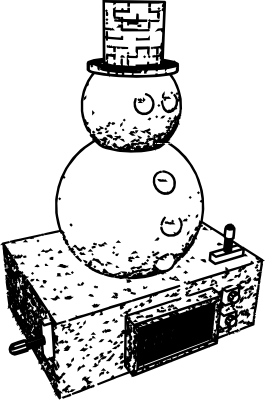
\includegraphics[scale=0.03]{rc/logo.png}}
\newcommand{\idx}[2]{#1 \index{#2@#1}}

% Au début de chaque section
\AtBeginSection[]{
	\begin{frame}[t]
		\frametitle{Nouvelle partie}
		\begin{block}{\Large \textbf{\insertsectionhead}}
			\textbf{Partie \thesection}
		\end{block}
	\end{frame}
}

% Les symboles dans les listes
\setbeamertemplate{itemize item}[ball]
\setbeamertemplate{itemize subitem}[triangle]
\setbeamertemplate{itemize subsubitem}[circle]

% Définit la 'profondeur' des tables des matières
\setcounter{tocdepth}{2}
% Active les coins arrondis et l'ombre pour les blocs d'information
\setbeamertemplate{blocks}[rounded][shadow=true]

\begin{document}

\begin{frame}[t,plain]
	\titlepage
\end{frame}

\begin{frame}[t]
	\frametitle{Sommaire}
	\tableofcontents
\end{frame}

\section{Général}

\begin{frame}[t]
	\frametitle{Idée initiale.}
	\begin{center}
		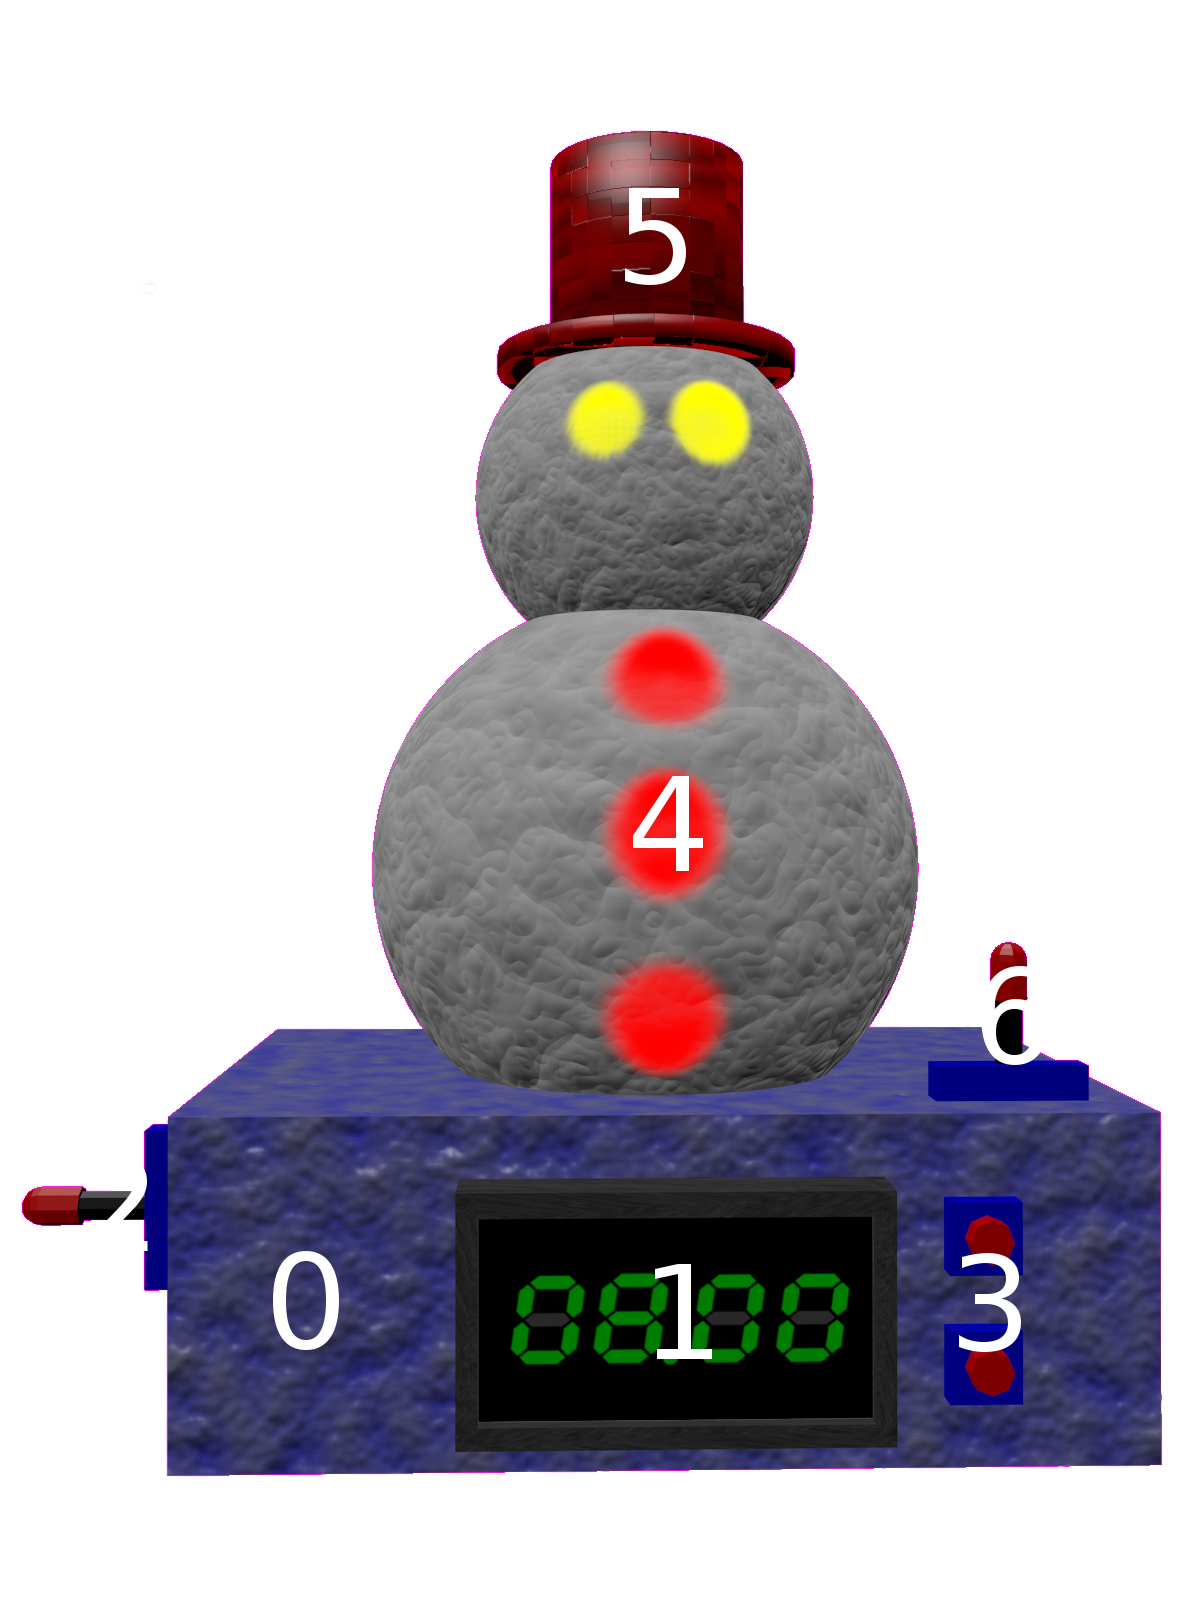
\includegraphics[scale=0.1]{rc/example_num.png}
	\end{center}
\end{frame}

\begin{frame}[t]
	\frametitle{Projet finit.}
	\begin{center}
		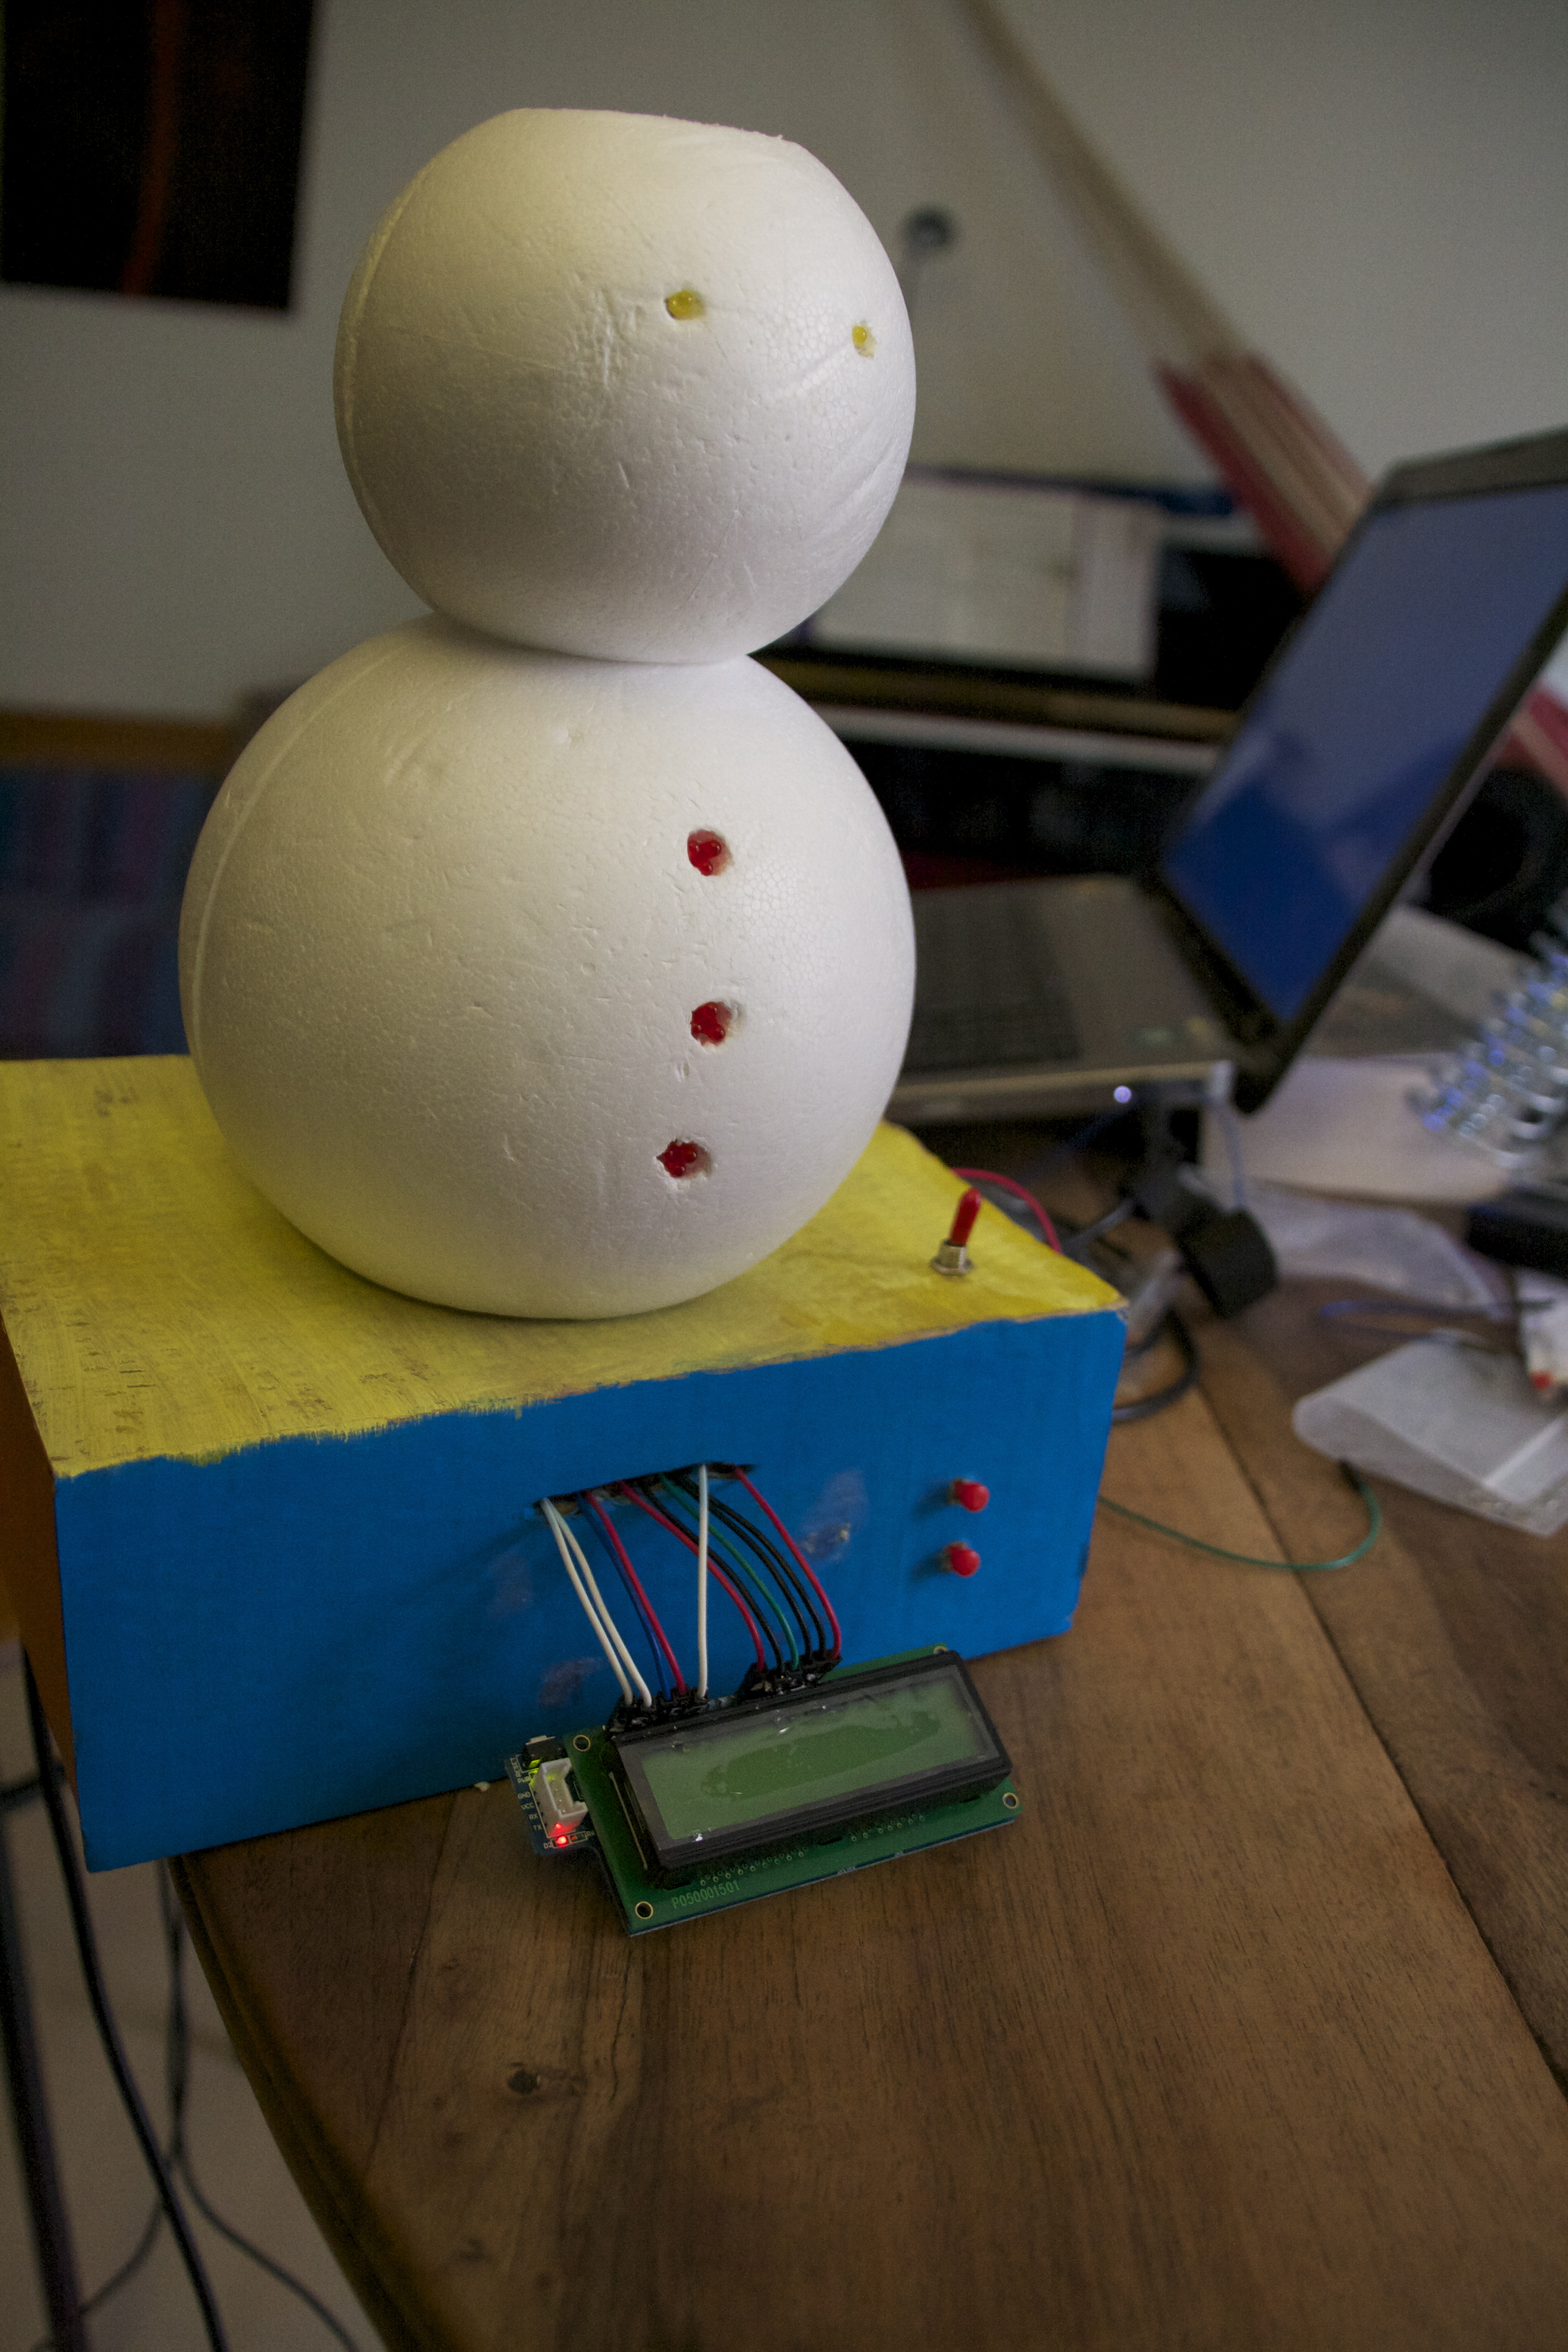
\includegraphics[scale=0.05]{rc/complet.jpg}
	\end{center}
\end{frame}

\section{Montage}

\begin{frame}
	\frametitle{Matériaux utilisés.}
	% Les matériaux (écran, carte arduino ...)
	\begin{FAST}{Snowy}
		\FT{Sonner}{ \ST{Speaker} }
		\FT{Réfléchir}{ \ST{Carte arduino} }
		\FT{Afficher l'heure}{ \ST{Écran} }
		\FT{Régler l'heure}{ \ST{Bouton poussoir}
		\ST{Interrupteur} }
		\FT{Stopper la sonnerie}{ \ST{Bouton poussoir} }
		\FT{Éclairer}{ \ST{LEDs} }
	\end{FAST}
\end{frame}

\begin{frame}
	\frametitle{Cablage.}
	\begin{center}
		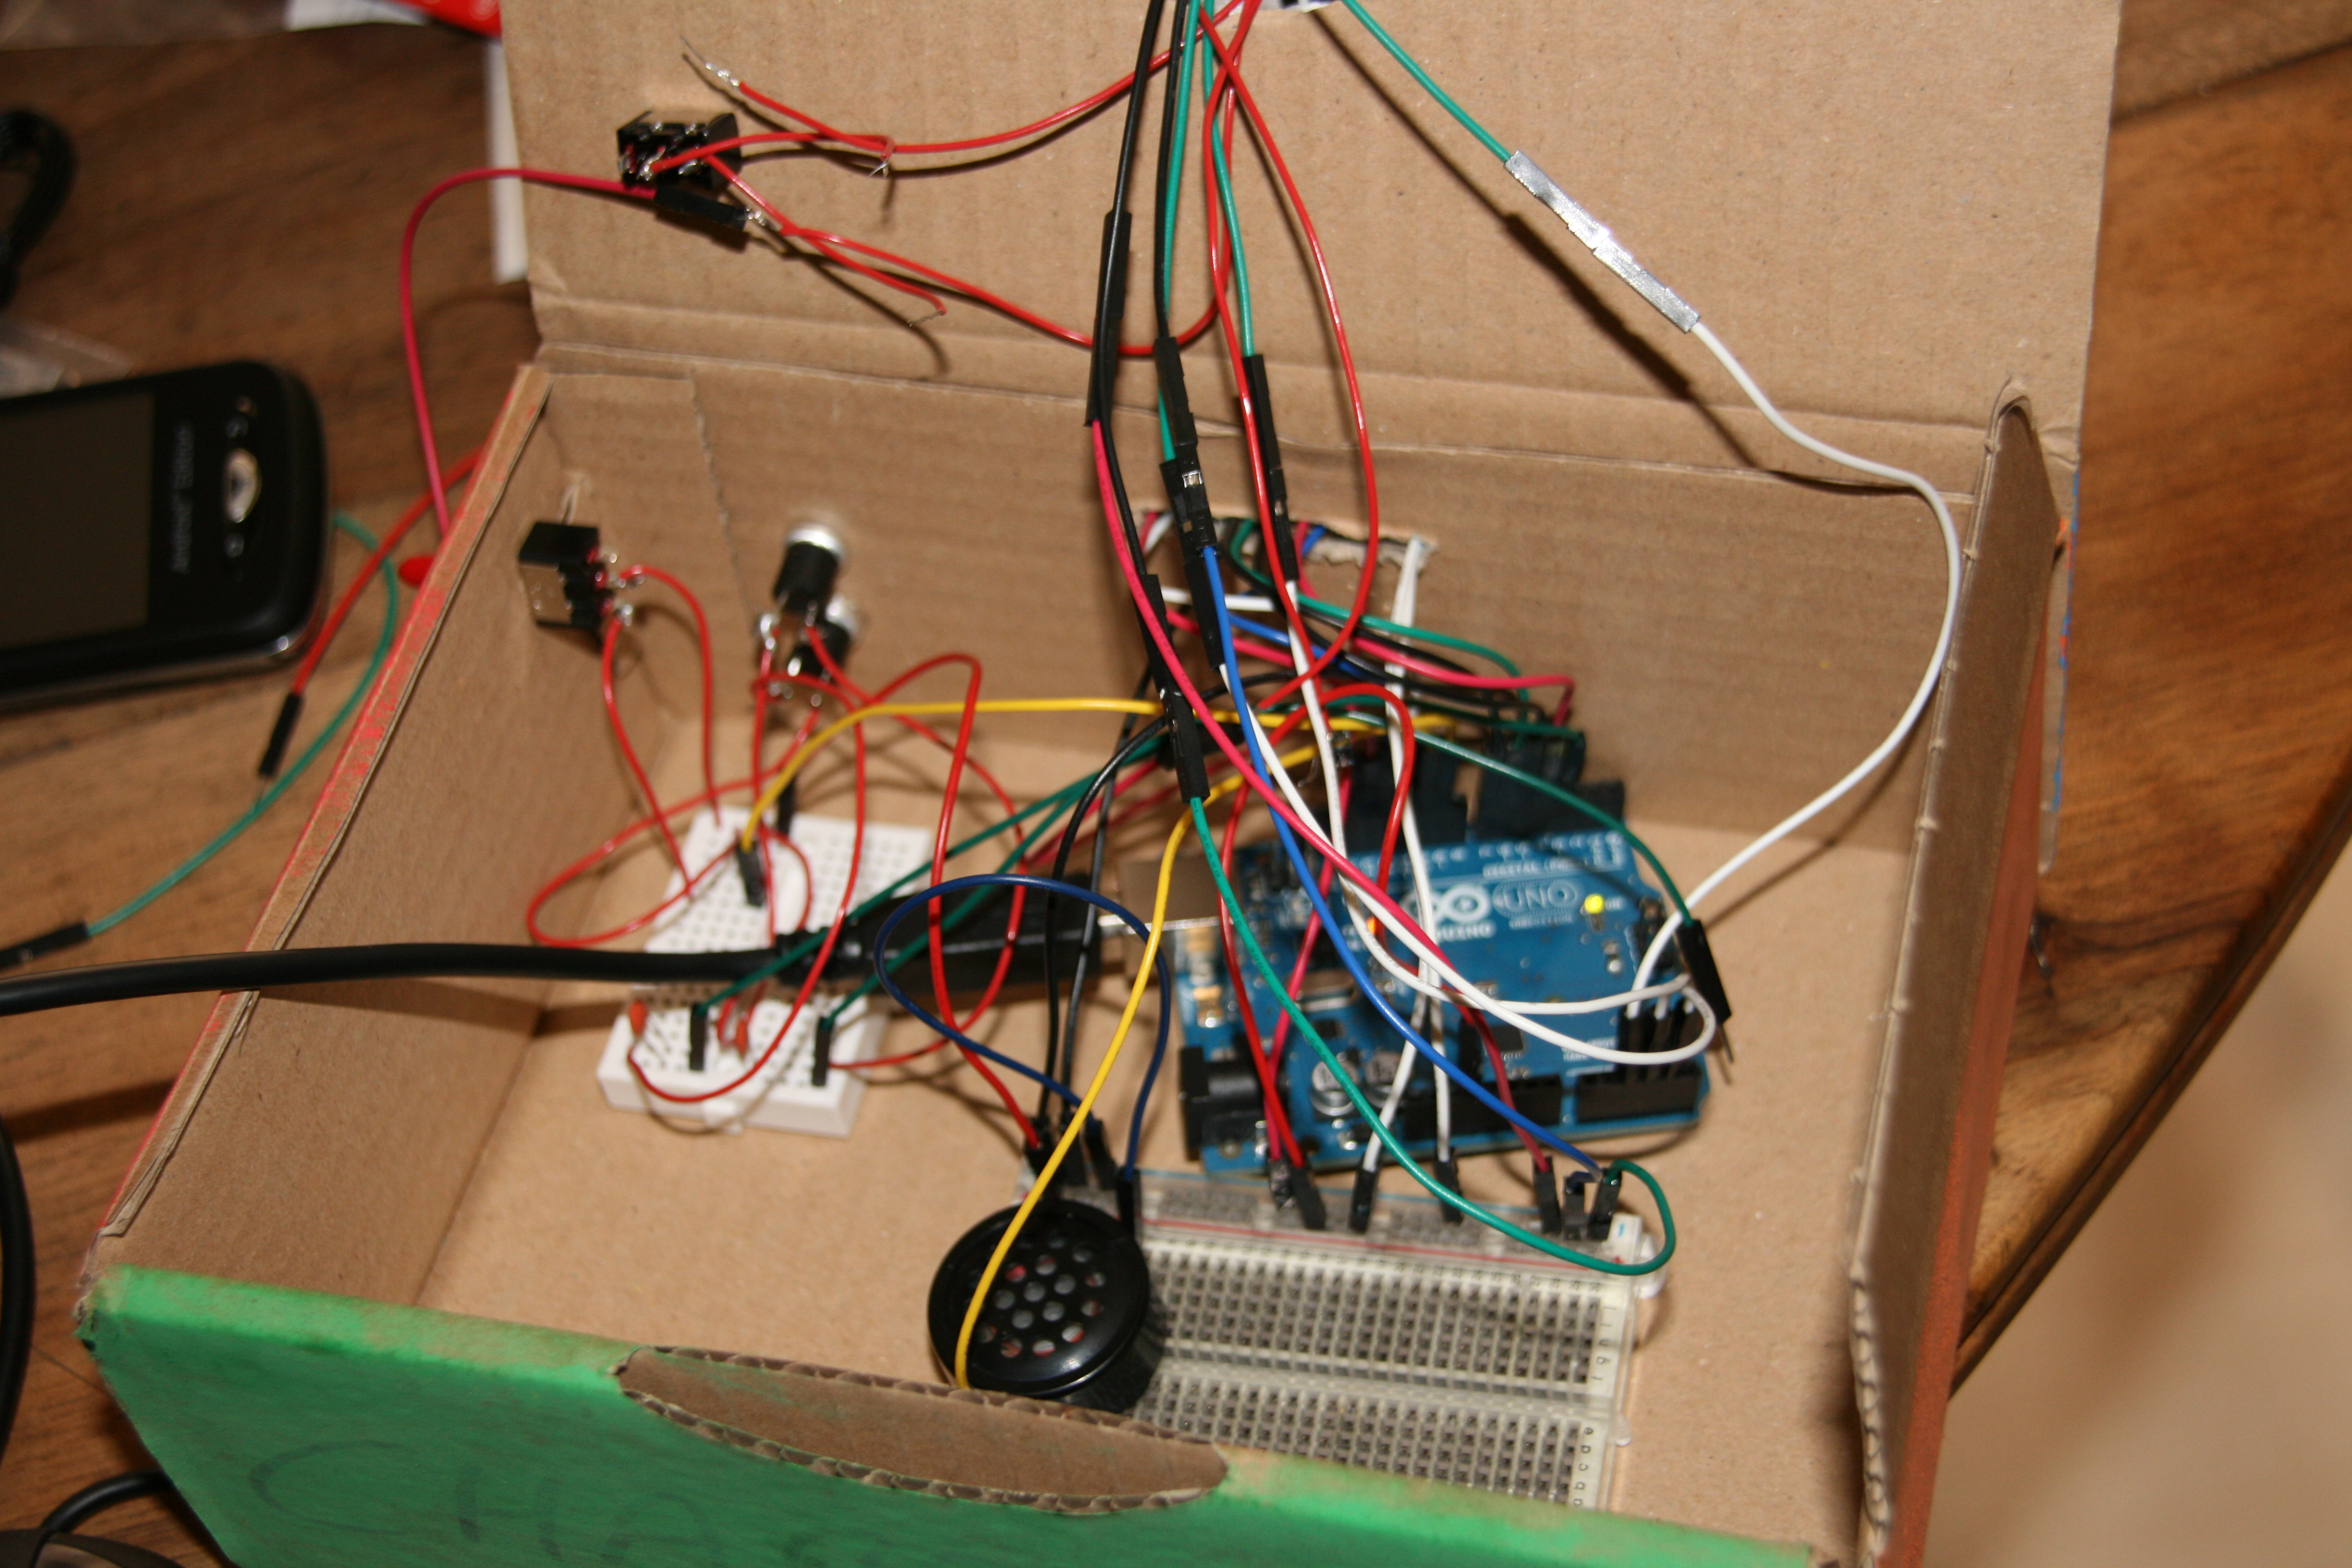
\includegraphics[scale=0.07]{rc/cablage.jpg}
	\end{center}
\end{frame}

\section{Programmation.}

\begin{frame}
	\frametitle{Architecture globale.}
	% UML
\end{frame}

\begin{frame}
	\frametitle{La mise à jour de l'heure.}
\end{frame}

\begin{frame}
	\frametitle{L'affichage de l'heure.}
\end{frame}

\begin{frame}
	\frametitle{La gestion des LEDs.}
\end{frame}

\begin{frame}
	\frametitle{Le son.}
\end{frame}

\section{Conclusion}

\begin{frame}
	\frametitle{Conclusion}
\end{frame}

\end{document}
